

\tikzset{every picture/.style={line width=0.75pt}} %set default line width to 0.75pt        

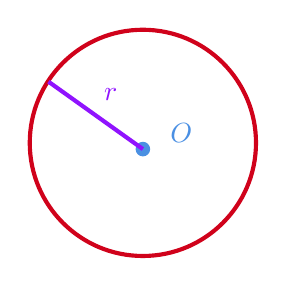
\begin{tikzpicture}[x=0.75pt,y=0.75pt,yscale=-1,xscale=1]
%uncomment if require: \path (0,140); %set diagram left start at 0, and has height of 140

%Shape: Circle [id:dp8118732481164563] 
\draw  [color={rgb, 255:red, 208; green, 2; blue, 27 }  ,draw opacity=1 ][line width=1.5]  (277,71.5) .. controls (277,41.4) and (301.4,17) .. (331.5,17) .. controls (361.6,17) and (386,41.4) .. (386,71.5) .. controls (386,101.6) and (361.6,126) .. (331.5,126) .. controls (301.4,126) and (277,101.6) .. (277,71.5) -- cycle ;
%Shape: Circle [id:dp14232976554180699] 
\draw  [color={rgb, 255:red, 74; green, 144; blue, 226 }  ,draw opacity=1 ][fill={rgb, 255:red, 74; green, 144; blue, 226 }  ,fill opacity=1 ] (328.5,74.5) .. controls (328.5,72.84) and (329.84,71.5) .. (331.5,71.5) .. controls (333.16,71.5) and (334.5,72.84) .. (334.5,74.5) .. controls (334.5,76.16) and (333.16,77.5) .. (331.5,77.5) .. controls (329.84,77.5) and (328.5,76.16) .. (328.5,74.5) -- cycle ;
%Straight Lines [id:da2079968527177969] 
\draw [color={rgb, 255:red, 144; green, 19; blue, 254 }  ,draw opacity=1 ][line width=1.5]    (286,42) -- (331.5,74.5) ;



% Text Node
\draw (350,67) node   {$\textcolor[rgb]{0.29,0.56,0.89}{O}$};
% Text Node
\draw (316,48) node   {$\textcolor[rgb]{0.56,0.07,1}{r}$};


\end{tikzpicture}